\begin{figure}[h]
  \label{fig:InequalityPFGICFHWCRIC}
  \centerline{
    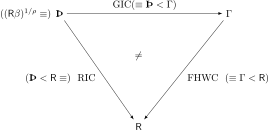
\includegraphics[width=3in]{\FigDir/InequalityPFGICFHWCRIC}
  }
  \caption{Relation of {\RIC}, {\GICRaw}, and {\FHWC} in Perfect Foresight Model}
  \footnotesize{Arrows reflect the direction of the relationship; an arrowhead points to the larger of the two quantities being compared.  For example, the topmost arrow, pointing from $\Pat$ to $\PGro$, indicates that $\PGro > \Pat$.}
\end{figure}
